% Prose copy of overleaf_draft.tex (bullet working draft left untouched).
% Needs in the preamble: \usepackage{amsmath, graphicx, booktabs, enumitem}

% ============================================================
% TODO — EXPERIMENTS STILL RUNNING (fill these in when they finish)
% ============================================================
%
% [RUNNING] E7/E10 secondary ablations (protocol-matched, 170 ep)
%            37 disc3d flatten   38 disc4d   39 discstack
%            40 perc=0.5         41 perc=3.0  42 kl=1e-7     (vs E1d 25.31)
%            43 LoRA rank 8      44 rank 128                 (vs E1c 31.21)
%            45 lora_before TC=on (E1d)  46 lora_before TC=off (E1c)
%            Historical wandb/April numbers are not cited (wrong protocol + LoRA load bug).
%
% DONE   E9b  512px fused+TC=on. Best val 26.64 dB / LPIPS 0.170 / Bleed-W 0.904 / XView 0.904
%            128: 25.31 → 256: 27.78 → 512: 26.64. The 128→256 lift does not continue.
%
% DONE   E_combo  temporal-diff-loss + 32-ch latent, fused+TC=on
%            job 5465204, 170 epochs. Best val: 29.56 dB / LPIPS 0.049 / Bleed-W 0.935
%            Delta +4.25 dB. Additive expect: 1.83+2.40 = 4.23 dB. They add.
% ============================================================

\section{Introduction}

% [feedback] object-centric framing established here, first paragraph, and kept consistent below
Photo-realistic head avatars are commonly built from synchronized multi-view facial video captured using dense camera rigs \cite{lombardi2018deep, lombardi2021mixture, cao2022authentic,
kirschstein2023nersemble, qian2024gaussianavatars}. Such rigs are object-centric: all cameras point at the same head from nearby positions, so their fields of view overlap almost completely. The captured video is therefore strongly redundant along two dimensions: \emph{time}, where adjacent frames differ by smooth facial motion, and \emph{view}, where nearby cameras observe overlapping facial regions with shared appearance and geometry \cite{taubner2025mvp4d, shah2024mv2mae}. (This premise matters: in a non-object-centric multi-camera setting, additional views add genuinely new content rather than redundancy, and nothing below applies.)


Modern generative pipelines do not operate on pixels, instead latent diffusion models generate in the compressed latent space of a Variational Auto Encoder (VAE) \cite{rombach2022high}, and video models such as Wan \cite{wan2025wan}, CogVideoX \cite{yang2024cogvideox}, HunyuanVideo \cite{kong2024hunyuanvideo} and Cosmos \cite{agarwal2025cosmos}, rely on a causal 3D video VAE that compresses space by 8x and time by 4x. Therefore, the tokenizer defines what the generator can express \cite{yu2024language}. If we want to generate, edit, or interpolate multi-view facial data with diffusion models, we first need a latent representation
of multi-view video. However, no such tokenizer exists: in recent work multi-view streams are encoded independently, which (i) leaves the massive view redundancy of object-centric capture uncompressed and (ii) provides no architectural prior for cross-view consistency, where each view's latent can drift independently under generation or editing.


% [feedback] "jointly learned" -> "jointly encoded": the point is that the ENCODER fuses the views.
% One could also encode views independently and let a diffusion model learn their correlations on a
% stacked 4D latent -- that is exactly the alternative we distinguish ourselves from.
This motivates a latent in which the views are jointly encoded: the encoder itself fuses the view axis into a single shared code, rather than encoding views independently and leaving their correlation to be modeled downstream (e.g. by a diffusion model trained on stacked per-view latents, as in current multi-view and 4D generation systems \cite{zuo2024videomv, xie2024sv4d}). Only joint encoding compresses the view redundancy and gives cross-view consistency by construction.
% [feedback] unambiguous: the extension concerns the VAE only, the diffusion model is untouched
Rather than designing a 4D VAE from scratch, we ask: can a pretrained 3D video VAE be minimally extended to absorb the view axis? Our changes concern the VAE only; the downstream diffusion model is untouched. We extend the Wan 2.1 VAE \cite{wan2025wan} with
zero-initialized multi-view self-attention fusion in the encoder and view-conditioned decoding via low-rank adapters \cite{hu2022lora, zhang2023adding}, keeping the pretrained backbone frozen so the latent remains compatible with unconditional sampling.
Through an extensive experimental study (32 configurations) on NeRSemble \cite{kirschstein2023nersemble} we find the following: the model reconstructs well when either the temporal axis is compressed (4$\times$, the native Wan setting: per-view PSNR 31.50~dB) or the view axis is fused into a shared latent (fused TC off: 31.21~dB), but combining both degrades quality super-additively (fused TC on: 25.31~dB --- a drop of 8.70~dB from the per-view reference, versus 5.31~dB predicted by the individual degradations; excess 3.39~dB). The failure is not architectural: swapping the fusion operator does not close the gap, and view-conditioning has no effect. It is also not a trainability artifact: full unfreezing makes things worse. It is a rate limit. This is consistent with the broader tokenizer literature, where reconstruction quality under higher compression is recovered by widening the latent channel dimension \cite{dai2023emu, chen2024deep, hacohen2024ltx}: widening from 16 to 32 channels recovers 2.40~dB --- our largest single gain --- confirming the diagnosis. Wider latents are known to complicate downstream generative modeling \cite{yao2025vavae}, so we study only the VAE side.
% [feedback] we CONFIRM the bottleneck, we do not remove it -- and we test the positive direction
% (widening) as an ablation on the VAE side, so the claim is not purely negative.
% RESOLVED: outcome is (b) partial recovery. Widening 16->32 gives +2.40 dB (E11a);
% 32->64 adds only 0.01 dB (E11b). A 3.79 dB gap to the per-view TC reference remains,
% attributable to the joint-view encoding challenge and frozen strided conv bottleneck.
% Framing: "capacity is necessary but not sufficient at adapter scale."
Our extension confirms this rate bottleneck rather than removing it: fusing a third axis into a latent sized for one collapses views toward their mean and frames within chunks toward their temporal mean. To verify that the limit is really the rate and not our architecture, we additionally widen the latent (16 to 32/64 channels, VAE-side only, no diffusion retraining): widening from 16 to 32 channels recovers 2.40~dB under joint compression --- the single largest gain in the study, larger than all architectural interventions combined --- providing direct positive evidence for the capacity interpretation.

Our contributions are as follows.
First, we give a minimal, weight-compatible extension of a pretrained 3D video VAE to synchronized multi-view video: zero-initialized multi-view self-attention in the encoder and per-view low-rank adapters in the decoder. At step 0 the model is near-identical to the pretrained per-view VAE; only the $V{\to}1$ merge introduces fresh weights.
Second, we run a controlled empirical study (32 configurations) of joint view and temporal compression at fixed latent width, holding data and budget fixed and varying only the compressed axes. Joint compression drops PSNR by 8.70~dB from the per-view reference, a super-additive 3.39~dB excess over what the individual degradations predict.
Third, we introduce two diagnostics that localize the failure --- cross-view similarity for ghosting and bleed ratio for temporal averaging --- separating it from generic reconstruction error, each anchored by a positive or negative control.
Fourth, we show that the failure is a rate and capacity limit, not a fusion-design or trainability problem: self-attention, channel Conv3d, and factorized 4D-conv fusion, plus five view-conditioning variants, all fail to close the joint-compression gap; full unfreezing of the network makes quality worse, not better; and widening the latent from 16 to 32 channels recovers 2.40~dB, the largest single improvement, directly confirming the capacity bottleneck.


\section{Related Work}

Although our target application is head avatar modeling from multi-view facial video, temporal and view redundancy are studied more broadly in the video representation learning literature, which we shortly review.
% [feedback] "The gap" is no longer a standalone subsection; each paragraph below ends with its own gap.

\subsection{Single-view video tokenizer}

Latent diffusion \cite{rombach2022high} was extended from images to videos either by inflating image autoencoders with temporal layers \cite{blattmann2023align} or by training causal 3D tokenizers \cite{yu2024language}. Video foundation models have since converged on a shared recipe: causal 3D convolutions, $8\times$ spatial and $4\times$ temporal compression, a 16-channel latent, and an L1+LPIPS+KL+GAN objective \cite{esser2021taming} carried over from images with little change \cite{wan2025wan, yang2024cogvideox, kong2024hunyuanvideo, agarwal2025cosmos}. These tokenizers are tuned to compress one or two axes of redundancy --- temporal motion at a fixed spatial rate --- and have no notion of view.

When multi-view data is passed through a standard video model it is encoded stream-wise. In the object-centric case (our setting) the streams are largely redundant, so this spends $V$ times the latent rate on content that is mostly shared. In a non-object-centric setting stream-wise encoding is appropriate, since each view carries new content. The gap is that these tokenizers have no view notion at all: nobody has asked what happens when a second compressed axis is added to their fixed latent budget. That is our experiment.

\subsection{Latent capacity}

The relevant question here is not which redundancy a tokenizer exploits, but how much compression a latent can support before quality degrades. Rombach et al.\ \cite{rombach2022high} already show this in the original LDM ablation, trading downsampling factor against channel count. Subsequent work makes the same point more sharply. Emu \cite{dai2023emu} keeps $8\times$ spatial compression and widens the latent from 4 to 16 channels so that small objects are reconstructed instead of lost. DC-AE \cite{chen2024deep} pushes compression up to $128\times$, but only with the channel count scaled alongside it: width is a necessary ingredient of the recipe, not the whole of it. LTX-Video \cite{hacohen2024ltx} buys $192\times$ spatiotemporal compression with a 128-channel latent, eight times the standard video-VAE width. VA-VAE \cite{yao2025vavae} is the counterpoint: wider latents do reconstruct better, but they are harder for a diffusion transformer to sample from, and the proposed fix is to align the latent with a frozen vision foundation model rather than keep widening. Collectively these papers show that one new axis of compression can be recovered by adding channels, at a cost on the generation side.

None of this asks what happens when the added axis is view rather than space or time, and none starts from a frozen pretrained latent rather than training from scratch. We measure both directions on a real pretrained backbone: at fixed 16-channel width, joint view and temporal compression collapses (25.31~dB vs.\ 31.50~dB per-view with temporal compression); widening the VAE latent from 16 to 32/64 channels, without retraining the diffusion model, recovers 2.40~dB --- positive evidence that the capacity interpretation extends to the view axis.

\subsection{Multi-view and 4D generation}

View consistency is typically solved architecturally, via cross-view attention, or geometrically, via explicit 3D. Cross-view attention is the default mechanism in multi-view diffusion \cite{shi2023mvdream, gao2024cat3d, voleti2024sv3d, zuo2024videomv}: every view attends to every other at generation time, which enforces consistency without compressing the views into a shared representation. MV2MAE \cite{shah2024mv2mae} reconstructs views from synchronized inputs via masked autoencoding, but the objective is reconstruction, not compression, and the resulting features are not a latent a generative model can sample from. 4D generation methods extend consistency to space, time, and view, but they rely on iterative sampling or explicit geometry \cite{zhang20244diffusion, xie2024sv4d, shao2024human4dit, jiang2026mesh4d}, again without producing a compact representation. Explicit geometry --- meshes, radiance fields, Gaussians \cite{qian2024gaussianavatars, kirschstein2023nersemble} --- makes consistency free because every view is a rendering of the same structure, yet there is no compact latent a diffusion model can sample from: the geometry itself is the object being modeled and edited, which is exactly what a generative model is supposed to abstract away. Pipelines for multi-view facial data \cite{lombardi2018deep, lombardi2021mixture} have the same limitation: they operate on pixels, per frame, with no latent space.

The gap is that all of these methods enforce view consistency at generation time or via geometry, but none provides a compact latent in which time and view are jointly compressed. Such a latent would be the natural substrate for a 4D generative model, which would be trained on it, and whose generated multi-view video would in turn feed reconstruction and avatar pipelines. That substrate is what we study.

\section{Methodology}

\subsection{Preliminaries: Wan 2.1 Video VAE}
\label{sec:preliminaries}

The Wan 2.1 VAE uses causal 3D convolutions, a 16-channel latent, and $8\times$ spatial / $4\times$ temporal compression. A video with $T$ frames maps to $T'$ latent frames,
\begin{equation}
T' = 1 + \left\lfloor \frac{T-1}{4} \right\rfloor,
\qquad
z \in \mathbb{R}^{16 \times T' \times H/8 \times W/8}
\label{eq:wan_latent}
\end{equation}
Temporal compression is implemented with a chunked feature cache: frame 0 is encoded and decoded alone, then the next 4 frames follow as one chunk, and so on. Each temporal convolution consumes a rolling cache from the previous chunk. Decoding mirrors this: one latent frame in, four frames out, with a persistent cache. Intra-chunk temporal bleeding, analyzed later, appears inside those four decoded frames.

% NOTE on all figure placeholders: they show the intended layout only. The actual result
% figures are produced after the reruns, from the best config -- mock versions for layout
% discussions live in paper/figures/ (make_mock_figures.py).
% [feedback] figure support for the chunk mechanism
\begin{figure}[t]
\centering
\fbox{\parbox[c][4.5cm][c]{0.9\linewidth}{\centering
PLACEHOLDER Fig.~\ref{fig:chunking}: timeline of the chunked cache mechanism.\\
Top row: input frames 0 | 1--4 | 5--8 grouped into chunks; arrows into latent frames $z_0, z_1, z_2$.\\
Bottom row: decode direction, one latent frame -> four output frames, cache arrows between chunks.\\
Highlight (color) where bleeding happens: within each decoded 4-frame group.}}
\caption{The causal chunked processing of the Wan 2.1 VAE. Frame 0 is processed alone, then 4-frame chunks with a rolling feature cache. One latent frame decodes to four output frames, which is where intra-chunk temporal bleeding appears.}
\label{fig:chunking}
\end{figure}

\subsection{Architecture: Multi-view extension}

% [feedback] formal support: notation + equations for the fusion and decoding path
Input is a synchronized multi-view clip $x \in \mathbb{R}^{V \times 3 \times T \times H \times W}$ with views $x_1, \dots, x_V$.

\begin{figure*}[t]
\centering
\fbox{\parbox[c][6cm][c]{0.95\linewidth}{\centering
PLACEHOLDER Fig.~\ref{fig:overview}: architecture overview (full width).\\
Left: V camera streams -> V frozen Wan encoder stems (drawn once, marked ``shared, frozen'').\\
Middle: multi-view self-attention block + binary tree merge -> single fused latent $z$ (16 ch).\\
Right: shared frozen decoder invoked V times, each pass with its per-view LoRA adapter -> V reconstructions.\\
Color code: blue = frozen pretrained, orange = new trainable (zero-init), green = LoRA.}}
\caption{Multi-view extension of the Wan 2.1 VAE. Views are encoded by the shared frozen per-view stem, fused at the bottleneck into a single latent, and decoded once per view with view-conditioned low-rank adapters. The attention and all LoRA paths are zero-initialized (identity at step 0); only the $V{\to}1$ merge blocks introduce fresh weights, since a many-to-one reduction has no identity configuration.}
\label{fig:overview}
\end{figure*}

\subsubsection{Design Decisions}

We adapt a pretrained 3D VAE rather than training a 4D VAE from scratch, in order to transfer pretrained knowledge \cite{carreira2017quo, blattmann2023align}, remain data-efficient, and keep the latent distribution close to the pretrained one. Every path that can be an identity at initialization is zero-initialized (the attention output projection and all LoRA up-projections). The only fresh weights are the $V{\to}1$ merge blocks, which have no identity configuration, so at step 0 the model is the pretrained per-view VAE up to the merge.

\subsubsection{Encoder-side cross-view fusion}

Each view passes through the frozen pre-fusion Wan encoder stem $E_{\mathrm{pre}}$, giving per-view bottleneck features
\begin{equation}
f_v = E_{\mathrm{pre}}(x_v) \in \mathbb{R}^{C_b \times T' \times h \times w},
\qquad C_b = 384,\; h = H/8,\; w = W/8 .
\end{equation}
Fusion operates at 384 channels on the $8\times$ downsampled grid: tokens are cheap for attention, but early enough that fused information still shapes the latent.

Multi-view self-attention treats all views' spatial positions at each latent time step as one token sequence (length $V \cdot hw$) and applies multi-head self-attention with a zero-initialized output projection $W_O$. (This is the mechanism that multi-view diffusion papers often call ``cross-view attention'' \cite{shi2023mvdream, gao2024cat3d}; we avoid that name since there is no query/key asymmetry between views.)
\begin{equation}
\tilde{f}_v = f_v + W_O \,\mathrm{MHA}\!\left(\mathrm{RMSNorm}([f_1, \dots, f_V])\right)_v ,
\qquad W_O = 0 \text{ at init,}
\label{eq:fusion_attn}
\end{equation}
so at step 0 the enriched features equal the per-view features. The $V$ enriched feature maps are then reduced to one by a binary tree of pairwise merges, each merge being a concatenation followed by two residual blocks:
\begin{equation}
m(a, b) = R_2\!\left(R_1\!\left([\,a ; b\,]\right)\right),
\qquad
g = m\big(\cdots m(\tilde{f}_1, \tilde{f}_2) \cdots\big) \in \mathbb{R}^{C_b \times T' \times h \times w},
\label{eq:tree_merge}
\end{equation}
and $g$ continues through the (LoRA-adapted) bottleneck middle/head of the pretrained encoder to produce the posterior, sampled with the usual reparameterization \cite{kingma2013auto}:
\begin{equation}
(\mu, \log \sigma^2) = \mathrm{split}\!\left(\mathrm{Conv}_{1\times1\times1}\!\left(E_{\mathrm{post}}(g)\right)\right),
\qquad
z = \mu + \sigma \odot \epsilon \;\in \mathbb{R}^{16 \times T' \times h \times w}.
\end{equation}

\begin{figure}[t]
\centering
\fbox{\parbox[c][5cm][c]{0.9\linewidth}{\centering
PLACEHOLDER Fig.~\ref{fig:fusion}: the three fusion mechanisms side by side (small schematics).\\
(a) multi-view self-attention + tree merge (ours, Eq.~\ref{eq:fusion_attn}--\ref{eq:tree_merge})\\
(b) channel-concat + 1x1x1 Conv3d + ResBlocks\\
(c) factorized (2+1+1)D convolution with a view-axis kernel}}
\caption{Fusion mechanisms compared in the ablation. All reduce V per-view feature maps to one shared map at the encoder bottleneck.}
\label{fig:fusion}
\end{figure}

\subsubsection{View-conditioned decoding}

The single fused latent is decoded V times by the shared frozen decoder $D$; view identity enters through per-view low-rank latent adapters (LoRA \cite{hu2022lora}, zero-init up-projection $B_v$):
\begin{equation}
\hat{x}_v = D\!\left(z + B_v A_v z\right),
\qquad
A_v \in \mathbb{R}^{r \times 16},\; B_v \in \mathbb{R}^{16 \times r},\; B_v = 0 \text{ at init.}
\label{eq:view_decode}
\end{equation}
An alternative (ablated) is a learned additive per-view embedding $e_v \in \mathbb{R}^{16}$.

\subsubsection{Trainable-parameter budget}

All remaining adaptation uses LoRA \cite{hu2022lora} on the frozen backbone with zero-initialized up-projections \cite{zhang2023adding}, i.e. every adapted weight is
\begin{equation}
W' = W + B A, \qquad B = 0 \text{ at init, } \operatorname{rank}(BA) \le r = 32.
\label{eq:lora}
\end{equation}
The pre-fusion per-view encoder stem is frozen. The bottleneck and the full decoder receive LoRA of rank 32 with zero-initialized up-projections; a limitation is that no LoRA path exists for strided convolutions. New fusion modules are trained fully. The strided temporal convolutions remain frozen.
% [feedback] overfit/training-discipline subsubsection removed from methods (kept as internal QA;
% the one-sequence-works-vs-many-fails observation appears in the experiments analysis instead)

\subsection{Objective}

The reconstruction term follows the standard latent-diffusion tokenizer recipe \cite{rombach2022high, zheng2024opensora} with a learned uncertainty weight $s$:
\begin{equation}
\mathcal{L} =
\frac{\lVert x - \hat{x} \rVert_1 + 1.5 \cdot \mathrm{LPIPS}(x, \hat{x})}{\exp(s)} + s
\;+\; 10^{-6} \cdot D_{\mathrm{KL}}\!\left(q(z \mid x) \,\Vert\, \mathcal{N}(0, I)\right).
\label{eq:objective}
\end{equation}
The KL term is always included, at weight $10^{-6}$, the standard tokenizer setting \cite{rombach2022high}, and is logged separately during training: the latent must stay a proper VAE posterior for downstream diffusion, not degrade into a plain autoencoder. An optional adversarial term uses one of three multi-view discriminator layouts, all PatchGAN-style 3D \cite{isola2017image}: views flattened into the batch, views stacked on channels, or an explicit 4D discriminator with a view axis and per-view embeddings.

% [feedback] "Data und Preprocessing" moved into the experiments section (merged with the dataset
% subsection there); val subject selection moved to the supplement.


\section{Experiments}

The training pipeline is adapted from Open-Sora's Wan finetuning, with multi-view data loading and per-view gradient checkpointing. Each run uses one L40S GPU.

% [added] overview first, so the reader sees the plan in one place
% [feedback] question-driven, not a sweep catalogue: every experiment answers one step of the
% argument; anything that does not carry the storyline goes to the supplement.
\subsection{Overview}

The experiments follow one line of reasoning.
Q1 asks whether joint view and temporal compression fails where single-axis compression does not; this is the main result (Tab.~\ref{tab:main}).
Q2 asks what fails: two failure modes, each with its own diagnostic, visualization, and experimental anchor --- view ghosting and temporal bleeding.
Q3 asks whether the failure is a design problem, via fusion-mechanism and view-conditioning ablations; if all variants fail alike, the design is not the bottleneck (Tab.~\ref{tab:fusion}, Tab.~\ref{tab:viewcond}).
Q4 asks whether it is trainability, by unfreezing up to the whole network; if a fully unfrozen model still fails, trainability is ruled out (Tab.~\ref{tab:unfreeze}).
Q5 asks whether it is capacity, the positive test: widen the latent from 16 to 32/64 under joint compression (Tab.~\ref{tab:width}), and add rate pressure via view count (Tab.~\ref{tab:views}) and generalization pressure via data scale (Fig.~\ref{fig:datascale}).

Secondary sweeps that tune the operating point but do not carry the argument (loss configuration, discriminator layouts, LoRA rank, initialization strategy, pre-fusion encoder LoRA) are kept in Sec.~secondary ablations for now and referred to from the analysis; once all results exist they may move to the supplement.

All numbers come from reruns under one fixed protocol; per-experiment configs are pinned in the repository.

\subsection{Experimental Setup}

\subsubsection{Dataset and preprocessing}
% [feedback] merged from the former methods Sec. "Data and Preprocessing"

We use NeRSemble \cite{kirschstein2023nersemble}: 16 synchronized cameras at 73~fps and $3208{\times}2200$, an object-centric head capture that is redundant along time (smooth facial motion) and view (neighboring cameras observe the same face). Preprocessing selects 8 frontal and upper-row cameras, temporally subsamples to 24~fps, then uniformly selects $T{=}9$ frames; applies the per-camera color correction provided with the dataset; center-square-crops; removes the background with RobustVideoMatting \cite{lin2022robust} composited on white; and bilinearly resizes to $\{128, 256, 512\}^2$. Clips are stored as $[V, T, C, H, W]$ in $[0,1]$ and trained as $[B, V, C, T, H, W]$ rescaled to $[-1,1]$ (full details in the supplement).

The main protocol uses $V{=}2$ synchronized frontal views, $T{=}9$ frames at $128{\times}128$, and one expression sequence per participant. $T{=}9$ maps to latent $T'{=}3$ (frame 0 plus two 4-frame chunks), so both bleeding within chunks and artifacts across a chunk boundary are measurable; $T{=}5$ has no chunk boundary at all. $V{=}2$ is the minimal view count, so any capacity failure can be traced to the joint representation itself rather than to an aggressive compression ratio, and it gives a clean $2\times$ rate factor against the per-view references. Larger view counts are studied as an explicit ablation later. Resolution $128{\times}128$ makes a controlled comparison of the full matrix affordable on single GPUs; resolution is scaled separately as its own check. Ten participants are held out entirely for validation (list in the supplement); all reported metrics are computed on these unseen identities. Unless stated otherwise, every experiment uses AdamW at learning rate $5{\times}10^{-4}$ (constant), bf16, effective batch 64, 170 epochs, LoRA rank 32, EMA 0.9999, and no discriminator.

\subsubsection{Comparability protocol}

% [added] comparability spelled out, this is what makes the tables defensible
The budget is defined in optimizer updates, not epochs or wall clock. Effective batch is fixed at 64 (micro-batch times accumulation, re-balanced automatically on memory limits). Every variant therefore sees the same number of updates and the same samples; all evaluations fire at the same update steps; no variant is early-stopped or extended individually. A plateau within the budget is the result, not a reason to train longer. Qualitative figures always show the same fixed participants, selected by dataset order and identical across variants, so grids are directly comparable between models.

\subsubsection{Metrics}

% [feedback] per metric: what it measures, how, why. Established metrics first, then our
% diagnostics. Disaggregated reporting instead of single averages.

Standard reconstruction quality: PSNR, SSIM, and LPIPS \cite{zhang2018unreasonable} on the held-out identities.

We report no single number averaged over everything. A global PSNR mean hides exactly the structure we care about, so PSNR is always disaggregated along one axis at a time. Per view, views are scored independently: ghosting pulls both decoded views toward their mean, degrading each view while a global average can still look plausible. Per frame index, averaged across views only, temporal failures have a signature over the frame index --- cold-start frame 0, dips at chunk boundaries, flattening within chunks. ``First frame good, later frames degraded'' is an insight; one scalar is not. The full per-axis profiles are plotted (Fig.~\ref{fig:perframe}); tables carry per-axis means.

Our diagnostics are reported for every arm. Each targets one failure mode and is calibrated against the ground truth. Established consistency metrics --- warping error \cite{lai2018learning}, VBench smoothness \cite{huang2024vbench}, epipolar TSED \cite{yu2023long}, MEt3R \cite{asim2025met3r}, re-rendering consistency \cite{gao2024cat3d}, FVD-V \cite{xie2024sv4d} --- are built for free generation and detect views or frames that disagree too much. Our failures are the opposite (views agreeing too much, frames changing too little) and would \emph{improve} those scores. We therefore measure the same axes calibrated against the paired GT, so deviation in either direction is visible.

Cross-view similarity (view ghosting) is the mean pairwise cosine similarity between decoded views of the same clip. The views are time-aligned by construction, so excess similarity is view mixing, not temporal structure. It is reported next to the same quantity on the GT views, following the pairwise-distance idea used to diagnose mode collapse in conditional generation \cite{zhu2017toward}, calibrated against GT. At the GT reference, views are decoded distinctly; above it, they ghost. The metric is experimentally anchored by the no-view-conditioning negative control (Tab.~\ref{tab:viewcond}), which must ghost.

Bleed ratio (temporal bleeding) is the mean $|f_{t+1}-f_t|$ of the reconstruction divided by the same quantity of the GT: the fraction of true motion the reconstruction reproduces. A value of 1 is faithful motion; well below 1 means frames are merged. It is computed separately within 4-frame chunks and across chunk boundaries, tying the artifact to the chunked causal decode (Sec.~\ref{sec:preliminaries}). It is anchored by the non-causal decode experiment (Tab.~\ref{tab:interventions}).

The anchor-drift profile is the mean $|f_k-f_0|$ for $k=1,\ldots,T{-}1$, GT versus reconstruction. The GT curve rises with $k$ as motion accumulates; a flat reconstruction curve means all frames stay too close to the clip start. This complements bleed ratio: consecutive-frame deltas miss a slow collapse toward a static clip, the anchored version does not. The per-frame-index error profile exposes cold-start and chunk-boundary artifacts.

View and temporal failure are disentangled by construction, not post hoc. The view metric compares across views at the same time step, so temporal structure cancels; the temporal metrics compare across time within the same view, so view identity cancels. Each is blind to the other failure mode. Each failure mode therefore has a measurement and an experimental anchor: ghosting has the negative control (must ghost), bleeding has the non-causal experiment (must not bleed). All diagnostic curves are plotted, not only averaged: a claim like ``bleeding'' must be visible in the plotted curves (Fig.~\ref{fig:perframe}); the scalars only summarize them.

\subsubsection{Reference points}

No like-for-like baseline exists, because nothing else produces a joint multi-view latent. Per-view models are therefore reported as reference points, not baselines: pretrained Wan zero-shot, and per-view LoRA-finetuned Wan. Both use $V$ times our latent rate and enforce no cross-view consistency, so all models are placed on a rate-quality plane instead of a single-rate ranking.

The floor is pretrained Wan zero-shot per view, with no training, which calibrates the domain gap to Wan's training distribution. The ceiling is per-view LoRA finetuning on all preprocessed data (all participants, all expressions; val identities excluded), with temporal compression off --- the best that ``just finetune Wan per view on our domain'' can do. It is deliberately not budget-matched (much more data, its own epoch count); it bounds the table from above and does not compete. It is evaluated on the same 10 val clips as every other row. The ceiling does not have to be perfect; it anchors what is achievable. The matched references are per-view LoRA finetuned on the same one-expression training set and budget as the fused arms; these are the controlled comparisons.

Compression ratio is $r = (V \cdot 3 \cdot T \cdot H \cdot W) / (V' \cdot C_z \cdot T' \cdot (H/8) \cdot (W/8))$ with $C_z = 16$. Our main configs span $r \in \{12{\times}/\text{view},\; 36{\times}/\text{view},\; 24{\times},\; 72{\times}\}$ for $V{=}2$, $T{=}9$, $H{=}W{=}128$ (per-view TC off / on, fused TC off / on); see Tab.~\ref{tab:main}.

\subsection{Main Results}

% [feedback] empty tables + example figures inserted for everything, so the story is visible
% before the numbers exist.

\begin{table}[t]
\centering
\caption{Main result: the rate-quality matrix. Per-view models are reference points at V times the latent rate, not baselines: the ceiling (per-view LoRA on all people and all expressions) bounds the table from above and is not budget-matched; the matched per-view rows share training data and budget with the fused arms. All rows are evaluated on the same 10 held-out identities (best-val EMA eval). PSNR is additionally reported per view and per frame index (Fig.~\ref{fig:perframe}); this table carries the per-axis means.}
\label{tab:main}
\begin{tabular}{llrrrrrr}
\toprule
Model & TC & Rate & PSNR $\uparrow$ & SSIM $\uparrow$ & LPIPS $\downarrow$ & XView sim & Bleed-W $\uparrow$ \\
\midrule
Wan zero-shot (per view, floor)      & off & 12$\times$/view & $\approx$21 & --     & --     & --    & -- \\
Per-view LoRA, all data (ceiling)    & off & 12$\times$/view & 34.34       & 0.9990 & 0.021  & 0.979 & 0.981 \\
Per-view finetuned (matched)         & off & 12$\times$/view & 34.01       & 0.9989 & 0.024  & 0.906 & 0.991 \\
Per-view finetuned (matched)         & on  & 36$\times$/view & 31.50       & 0.9981 & 0.041  & 0.907 & 0.952 \\
Fused latent (ours)                  & off & 24$\times$       & 31.21       & 0.9980 & 0.044  & 0.907 & 0.974 \\
\textbf{Fused latent (ours)}         & \textbf{on}  & \textbf{72$\times$} & \textbf{25.31} & \textbf{0.9917} & \textbf{0.082} & \textbf{0.920} & \textbf{0.919} \\
\midrule
GT reference level                   & --  & --              & --          & --     & --     & 0.907 & 1.0 \\
\bottomrule
\end{tabular}
\smallskip\\
\textit{Note: SSIM lies in the narrow range 0.991--0.999 for all non-broken configurations at 128$^2$; it is reported for completeness but is not discriminative at this resolution. Rate = (V$\cdot$3$\cdot$T$\cdot$H$\cdot$W)$/$(V'$\cdot$16$\cdot$T'$\cdot$(H/8)$\cdot$(W/8)) with T=9, T'=3 (TC=on) or T'=9 (TC=off), V=2, H=W=128.}
\end{table}

\begin{figure}[t]
\centering
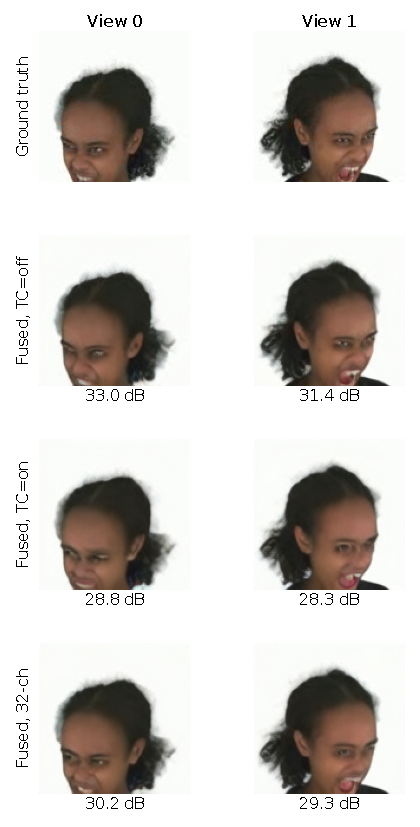
\includegraphics[width=\linewidth]{figures/qual_ghosting.pdf}
\caption{Same identity, two cameras. Joint compression (TC=on) blurs view-specific structure (hair parting, mouth). Widening the latent recovers some of it.}
\label{fig:qualitative}
\end{figure}

\begin{figure}[t]
\centering
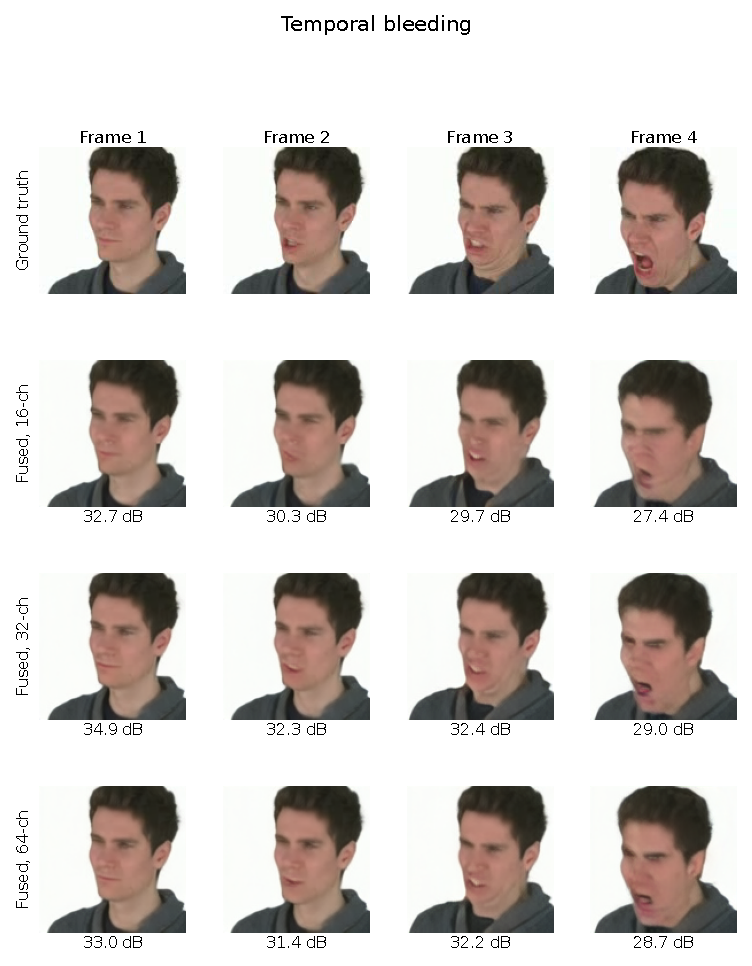
\includegraphics[width=\linewidth]{figures/qual_bleeding.pdf}
\caption{Temporal bleeding inside one 4-frame decode chunk. Numbers under each reconstruction are PSNR of that frame. Ground truth goes from closed mouth to a full scream; the 16-channel fused model averages toward a half-open mouth. Widening the latent restores more of the motion.}
\label{fig:qual_bleeding}
\end{figure}

\begin{figure}[t]
\centering
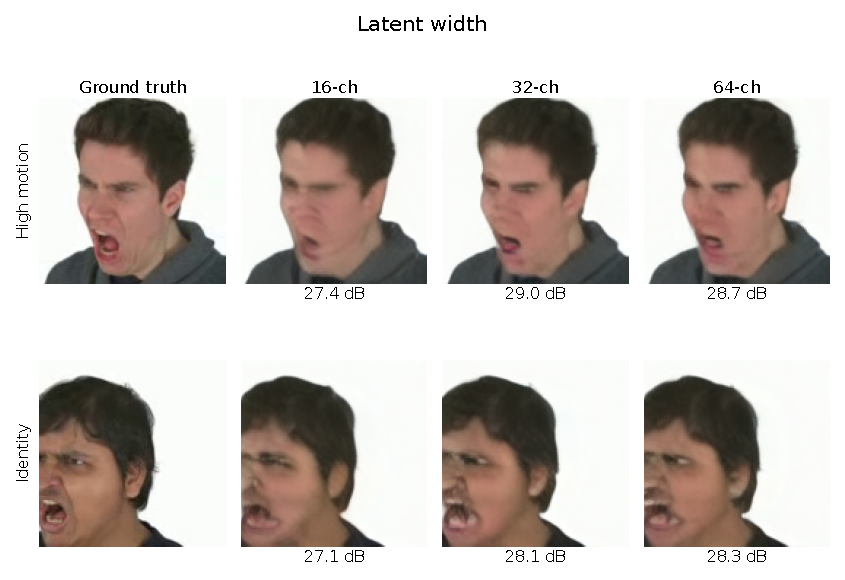
\includegraphics[width=0.92\linewidth]{figures/qual_capacity.pdf}
\caption{Latent width under joint compression. Numbers under each reconstruction are PSNR of that frame. 16 channels wash out teeth and brows; 32 channels restore them; 64 channels look the same as 32, matching Tab.~\ref{tab:width}.}
\label{fig:qual_capacity}
\end{figure}

Reading Tab.~\ref{tab:main}, the domain gap is visible in the ceiling row (34.34~dB, all data) versus the matched per-view reference (34.01~dB, same budget). The gap is small (0.33~dB), confirming that the one-expression training set already covers the val distribution well. Single-axis compression degrades gracefully: per-view temporal compression costs 2.51~dB ($34.01{\to}31.50$); view fusion alone costs 2.80~dB ($34.01{\to}31.21$). Critically, the fused TC-off model (31.21~dB at $24\times$) nearly matches the per-view TC-on model (31.50~dB at $36\times$/view), showing that the view axis can be absorbed at comparable rate-quality efficiency. Joint compression (fused TC on, $72\times$) drops to 25.31~dB: an 8.70~dB total drop, versus 5.31~dB predicted by summing the individual degradations. The excess 3.39~dB is super-additive: the two axes interfere. Both failure modes activate: bleed ratio drops to 0.919 (temporal bleeding) and cross-view similarity rises to 0.920, slightly above the GT reference of 0.907 (mild view ghosting). The 16-channel latent stores $3{\cdot}8{\cdot}8{\cdot}4/16 = 48\times$ per view natively; fusing $V{=}2$ doubles this to $96\times$ effective information density at fixed width. The failure is exactly what this predicts.



\subsection{Failure mode 1: view ghosting}

The failure modes are analyzed separately because the diagnostics separate them by construction (Sec.~metrics): the view metric cancels temporal structure, the temporal metrics cancel view identity.

The symptom is that decoded views drift toward their mean: high-frequency, view-specific detail is averaged away. This is visible in the qualitative grids (Fig.~\ref{fig:qualitative}) and measured as cross-view similarity above the GT reference (Tab.~\ref{tab:main}). Per-view PSNR drops for both views together --- ghosting is a symmetric collapse, not one view winning --- which is why quality is reported per view, not as one mean. The negative control without any view conditioning must ghost fully (Tab.~\ref{tab:viewcond}); the distance between our model and this control is the calibrated size of the effect.

Is it the conditioning? We compare per-view latent LoRA, a learned view embedding, and both (Tab.~\ref{tab:viewcond}). If all conditioned variants land in the same place, the conditioning mechanism is not what limits view separation. Is it the fusion design? We compare three fusion mechanisms with different inductive biases (Tab.~\ref{tab:fusion}, Fig.~\ref{fig:fusion_ablation}): multi-view self-attention with tree merge (default), channel-concat Conv3d, and factorized $(2{+}1{+}1)$D convolution. If ghosting appears across all of them, the fusion design is not the bottleneck. Comparing ghosting under TC off versus TC on separates ``view fusion is hard'' from ``view fusion is hard on top of temporal compression''.

The fusion variants in Tab.~\ref{tab:fusion} are as follows. Multi-view self-attention with tree merge (default) applies MHA over the concatenated token sequence of all views, with a zero-init output projection, then a pairwise tree merge (Eq.~\ref{eq:fusion_attn}--\ref{eq:tree_merge}). Channel-concat Conv3d stacks views on channels, followed by a $1{\times}1{\times}1$ Conv3d, GN/SiLU, and two symmetric (non-causal) 3D residual blocks. Factorized 4D convolution applies a spatial $3{\times}3$ Conv2d, a temporal $3{\times}3{\times}3$ Conv3d, then a view-axis Conv3d with kernel $(V,3,3)$ compressing $V{\to}1$. The view-conditioning variants in Tab.~\ref{tab:viewcond} are per-view latent LoRA adapters (default), a learned per-view latent embedding $e_v\in\mathbb{R}^{16}$ added to $z$, both combined, and the no-conditioning negative control.



\subsection{Failure mode 2: temporal bleeding}

The symptom is that frames within a 4-frame decode chunk merge: motion is under-reproduced inside chunks while chunk boundaries stay comparatively sharp. This is measured by the within/across bleed-ratio split and the anchor-drift profile, plotted per frame index (Fig.~\ref{fig:perframe}). It is also a generalization failure: overfitting a single sequence is clean, and artifacts appear only when many identities are trained, so the compressed representation can memorize temporal detail but cannot encode it for new content (Fig.~\ref{fig:datascale}).

A natural intuition is that decoding all latent frames in a single non-causal pass should remove frame-0 and boundary artifacts, bounding how much causal chunking itself costs. In practice, switching pretrained causal convolutions to symmetric padding catastrophically disrupts pretrained feature statistics (17.81~dB, bleed ratio 0.251). This is a negative finding, not an oracle; the non-causal path requires retraining from scratch with non-causal convolutions, which is out of scope.

Targeted interventions (Tab.~\ref{tab:interventions}, Fig.~\ref{fig:interventions}) attack hypothesized causes with four baseline-preserving flags. Reflection padding, a learned cache update, and a sub-frame position embedding each improve PSNR by 0.57--0.65~dB, within noise at the one-seed level. The temporal-difference loss (+1.83~dB) is the decisive outlier among 16-channel runs: directly penalizing L1$(\Delta\mathrm{gt}, \Delta\mathrm{rec})$ forces the model to preserve inter-frame differences even under latent averaging pressure. Combining it with the learned cache update does not stack (+1.62~dB), suggesting they compete for the same degrees of freedom. Combining it with a 32-channel latent does: E\_combo reaches 29.56~dB (${+}4.25$~dB), matching the ${+}4.23$~dB sum of the two isolated gains, so the loss and the extra channels address independent constraints. The temporal-difference loss reduces LPIPS from 0.082 to 0.070; E\_combo further to 0.049. We do not consider pixel-to-decoder skip connections: they would require the input video at decode time and are incompatible with unconditional generation from a sampled latent.

\begin{figure}[t]
\centering
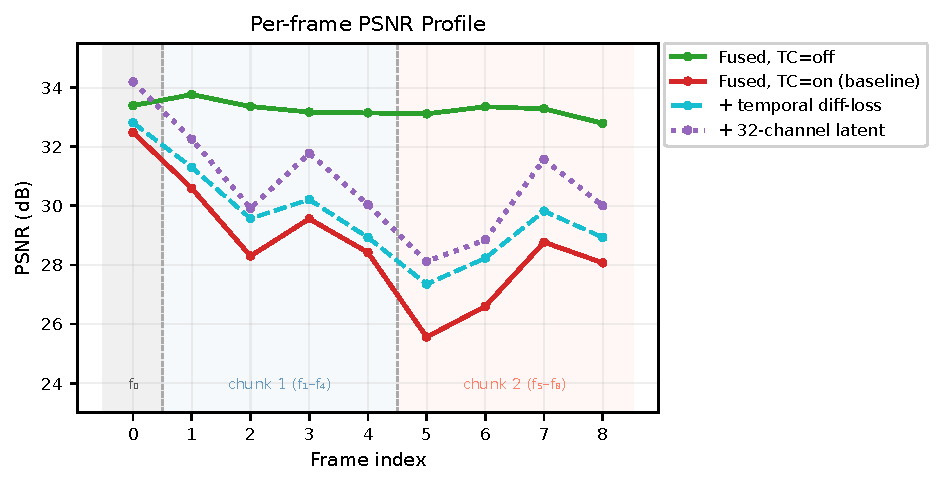
\includegraphics[width=\linewidth]{figures/perframe_psnr.pdf}
\caption{Per-frame PSNR on held-out identities. Without temporal compression the profile is flat. With it, quality drops inside each 4-frame decode chunk (f$_1$--f$_4$, f$_5$--f$_8$). A temporal-difference loss and a 32-channel latent both lift the troughs without removing the chunk structure.}
\label{fig:perframe}
\end{figure}

\begin{figure}[t]
\centering
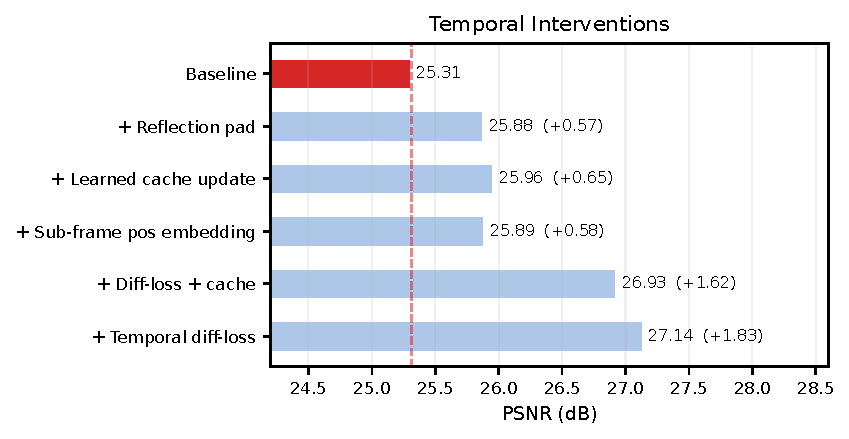
\includegraphics[width=0.95\linewidth]{figures/interventions.pdf}
\caption{Temporal interventions under joint compression. Architectural tweaks to padding, the feature cache, and sub-frame identity give only small gains; supervising inter-frame differences is the only 16-channel intervention that moves the needle. Combining that loss with a 32-channel latent is additive.}
\label{fig:interventions}
\end{figure}

\begin{table}[t]
\centering
\caption{Temporal interventions under joint compression (fused, TC on). The non-causal decode (E4b) is \emph{not} an oracle: permanently switching pretrained causal convolutions to symmetric padding collapses quality catastrophically. The temporal-difference loss (E4h$^\star$) is the only decisive 16-channel intervention; combining it with a 32-channel latent is additive.}
\label{tab:interventions}
\begin{tabular}{lrrrr}
\toprule
Intervention & PSNR $\uparrow$ & $\Delta$ & Bleed-W $\uparrow$ & LPIPS $\downarrow$ \\
\midrule
none (baseline)                             & 25.31 & 0       & 0.919 & 0.082 \\
non-causal decode (E4b) $\dagger$           & 17.81 & $-$7.50 & 0.251 & 0.187 \\
\midrule
temporal reflection pad                     & 25.88 & $+$0.57 & 0.899 & 0.070 \\
learned cache update                        & 25.96 & $+$0.65 & 0.899 & 0.069 \\
sub-frame position embedding                & 25.89 & $+$0.58 & 0.896 & 0.069 \\
\textbf{temporal-diff.\ loss$^\star$}       & \textbf{27.14} & $\mathbf{+}$\textbf{1.83} & \textbf{0.903} & \textbf{0.070} \\
diff.\ loss + learned cache                 & 26.93 & $+$1.62 & 0.899 & 0.069 \\
\midrule
\textbf{diff.\ loss + 32-ch latent}         & \textbf{29.56} & $\mathbf{+}$\textbf{4.25} & \textbf{0.935} & \textbf{0.049} \\
\bottomrule
\multicolumn{5}{l}{\small $\dagger$ catastrophic failure: disrupts pretrained causal feature statistics.}\\
\multicolumn{5}{l}{\small $^\star$ best 16-channel intervention; does not stack with the learned cache update.}\\
\multicolumn{5}{l}{\small Diff.\ loss ${+}1.83$ and 32-ch ${+}2.40$ add: ${+}4.25$ vs.\ ${+}4.23$ expected.}\\
\end{tabular}
\end{table}



\subsection{Is it capacity? Trainability, width, and rate pressure}


\subsubsection{Trainability check: unfreezing}

Strided temporal convolutions allow no LoRA path and are frozen in all LoRA configurations, so we unfreeze them and optionally the full encoder or full decoder. If even full unfreezing does not fix joint compression, the bottleneck is capacity, not trainability (Tab.~\ref{tab:unfreeze}).

\subsubsection{Latent width: the positive capacity test}
% RESOLVED: partial recovery (framing b). E11a (+2.40 dB) is decisive; E11b adds 0.01 dB.
% Capacity is necessary but not sufficient at adapter scale.

We widen the latent from the pretrained 16 channels to 32 and 64 under joint compression (fused + TC), following the width recipes of \cite{dai2023emu, chen2024deep, hacohen2024ltx}. Only four convolutions in the whole network touch the latent width: the encoder's final head conv ($384 \to 2C_z$), the two $1{\times}1$ latent convs around the sampling step, and the decoder's input conv ($C_z \to 384$). Everything else, including the encoder/decoder middle blocks and the attention in the encoder head, operates at 384 channels and is reused completely unchanged; widening does not discard any interior pretrained weights. On the four boundary convs, the pretrained 16-channel kernels occupy the first 16 slots; new output channels start at zero (emit nothing) and new input channels have zero weight (ignored), in the spirit of \cite{zhang2023adding}, so at step 0 the widened model computes exactly the 16-channel model. The four boundary convs are unfrozen ($\approx$2M params, still adapter-scale); there is no diffusion retraining.

The result (Tab.~\ref{tab:width}) is that $16{\to}32$ channels yields ${+}2.40$~dB (27.71 vs.\ 25.31~dB), the single largest isolated gain in the study. $32{\to}64$ channels adds ${+}0.01$~dB (no further benefit). Bleed ratio improves modestly (0.930 vs.\ 0.919), confirming that temporal artifacts partly reflect latent overcrowding. A 3.79~dB gap to the per-view TC reference (31.50~dB) remains at 32 channels alone: capacity is necessary but not sufficient at adapter scale; the frozen temporal convolutions and the joint-view encoding challenge account for the remainder.

Training the temporal-difference loss on the 32-channel model tests whether those two remaining constraints are the same constraint. They are not: E\_combo reaches 29.56~dB (${+}4.25$~dB over the 16-channel joint baseline), within 0.02~dB of the ${+}4.23$~dB sum of the isolated effects. The leftover gap to the per-view TC reference shrinks from 3.79~dB to 1.94~dB. Width and temporal supervision are complementary, not substitutes.

\begin{table}[t]
\centering
\caption{Latent-width ablation under joint compression (fused, TC on). Widening from 16 to 32 channels (+2.40~dB) is the single largest gain in the study — direct positive evidence that the 16-channel rate is the binding constraint.}
\label{tab:width}
\begin{tabular}{lrrrrr}
\toprule
Latent channels & Rate & PSNR $\uparrow$ & LPIPS $\downarrow$ & XView sim & Bleed-W $\uparrow$ \\
\midrule
16 (pretrained, E1d)         & 72$\times$  & 25.31 & 0.082 & 0.920 & 0.919 \\
\textbf{32 (E11a$^\star$)}   & 36$\times$  & \textbf{27.71} & \textbf{0.062} & \textbf{0.908} & \textbf{0.930} \\
64 (E11b)                    & 18$\times$  & 27.60 & 0.063 & 0.908 & 0.921 \\
\midrule
Per-view TC=T ref.\ (E1b)    & 36$\times$/view & 31.50 & 0.041 & 0.907 & 0.952 \\
\bottomrule
\multicolumn{6}{l}{\small Rate $= (V{\cdot}3{\cdot}T{\cdot}H{\cdot}W) / (V'{\cdot}C_z{\cdot}T'{\cdot}(H/8){\cdot}(W/8))$, V=2, T=9, H=128.}\\
\multicolumn{6}{l}{\small $^\star$ 16$\to$32 and 16$\to$64 yield the same rate as E1b, but 3.8~dB below it: the joint view encoding still costs.}\\
\end{tabular}
\end{table}

\begin{figure}[t]
\centering
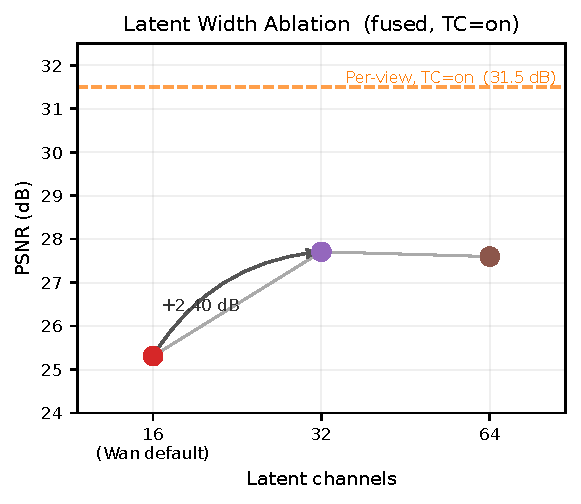
\includegraphics[width=0.72\linewidth]{figures/latent_width.pdf}
\caption{Widening the fused TC-on latent from the Wan default of 16 channels to 32 recovers +2.40~dB. Doubling again to 64 channels adds nothing: the first doubling is the capacity that was missing; beyond that a secondary bottleneck dominates.}
\label{fig:latent_width}
\end{figure}

\begin{figure}[t]
\centering
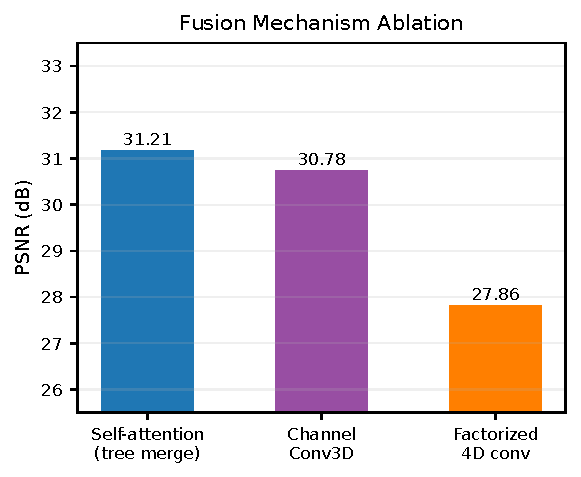
\includegraphics[width=0.78\linewidth]{figures/fusion_ablation.pdf}
\caption{Fusion-operator ablation under view fusion without temporal compression. Self-attention with tree merge and channel Conv3d are equivalent; a factorized 4D conv is worse. The joint-compression failure is therefore not an artifact of the default fusion design.}
\label{fig:fusion_ablation}
\end{figure}

\begin{table}[t]
\centering
\caption{Fusion mechanism ablation (fused latent, TC off). Self-attention and channel Conv3d land within 0.43~dB of each other; the factorized 4D conv underperforms. Near-equivalence of the competitive operators is itself evidence that the bottleneck is latent capacity, not fusion design. Bottom row: the default operator re-run with TC on.}
\label{tab:fusion}
\begin{tabular}{llrrrr}
\toprule
TC & Fusion & PSNR $\uparrow$ & LPIPS $\downarrow$ & XView sim & Bleed-W $\uparrow$ \\
\midrule
off & self-attn + tree merge (default) & 31.21 & 0.044 & 0.907 & 0.974 \\
off & channel-concat Conv3d           & 30.78 & 0.041 & 0.979 & 0.966 \\
off & factorized (2+1+1)D conv        & 27.86 & 0.073 & 0.979 & 0.927 \\
\midrule
on  & self-attn + tree merge (default) & 25.31 & 0.082 & 0.920 & 0.919 \\
\bottomrule
\end{tabular}
\end{table}

\begin{table}[t]
\centering
\caption{View-conditioned decoding (fused latent, TC off). All variants lie within 0.21~dB of each other, including the negative control (no conditioning at all). Cross-view attention implicitly encodes sufficient view identity; explicit conditioning adds no measurable gain.}
\label{tab:viewcond}
\begin{tabular}{lrrr}
\toprule
Conditioning & PSNR $\uparrow$ & LPIPS $\downarrow$ & XView sim (GT: 0.978) \\
\midrule
per-view latent LoRA, default (E1c) & 31.21 & 0.044 & 0.907 \\
view embedding only (E3a)           & 31.53 & 0.036 & 0.979 \\
view embedding + LoRA (E3c)         & 31.37 & 0.037 & 0.979 \\
full decoder finetune (E3e)         & 31.32 & 0.038 & 0.978 \\
\textbf{none} (negative control, E3d) & \textbf{31.50} & \textbf{0.037} & \textbf{0.979} \\
\bottomrule
\multicolumn{4}{l}{\small Negative control reconstructs distinct views without any explicit view signal;}\\
\multicolumn{4}{l}{\small cross-view attention alone encodes view identity. Max spread: 0.32~dB.}\\
\end{tabular}
\end{table}

\begin{table}[t]
\centering
\caption{Freezing ablation (fused, TC on). Full unfreezing makes quality \emph{worse} ($-$1.42~dB), ruling out adaptation constraint as the cause of joint-compression failure.}
\label{tab:unfreeze}
\begin{tabular}{lrrrr}
\toprule
Trainable scope & PSNR $\uparrow$ & $\Delta$ & Bleed-W $\uparrow$ & LPIPS $\downarrow$ \\
\midrule
LoRA only (default, E1d)           & 25.31 & 0       & 0.919 & 0.082 \\
+ full encoder unfrozen (E5b)       & 25.88 & $+$0.57 & 0.915 & 0.083 \\
+ full decoder, nothing frozen (E5c) & 23.89 & $-$1.42 & 0.886 & 0.123 \\
\bottomrule
\multicolumn{5}{l}{\small Full unfreezing: decoder overfits on our dataset scale, worsening generalization.}\\
\multicolumn{5}{l}{\small Frozen-bottleneck confound ruled out: adding parameters hurts, not helps.}\\
\end{tabular}
\end{table}




\subsubsection{Rate pressure: number of views}

We vary $V \in \{2,4,8\}$ at fixed budget and fixed fusion mechanism. Rate pressure on the shared latent grows with $V$, so we expect monotone degradation and earlier onset of ghosting.

\begin{table}[t]
\centering
\caption{View count ablation (fused latent, self-attn, TC off and on). Quality degrades monotonically with view count at both settings, consistent with growing rate pressure on the fixed 16-channel latent. At TC on, 8-view shows simultaneous severe bleeding (Bleed-W 0.755) and ghosting (XView sim above GT).}
\label{tab:views}
\begin{tabular}{llrrrr}
\toprule
TC & V & Rate & PSNR $\uparrow$ & LPIPS $\downarrow$ & Bleed-W $\uparrow$ \\
\midrule
off & 2 (E1c)  & 24$\times$  & 31.21 & 0.044 & 0.974 \\
off & 4 (E6b)  & 48$\times$  & 28.00 & 0.061 & 0.954 \\
off & 8 (E6d)  & 96$\times$  & 25.15 & 0.111 & 0.927 \\
\midrule
on  & 2 (E1d)  & 72$\times$   & 25.31 & 0.082 & 0.919 \\
on  & 4 (E6c)  & 144$\times$  & 23.23 & 0.101 & 0.837 \\
on  & 8 (E6e)  & 288$\times$  & 20.25 & 0.152 & 0.755 \\
\bottomrule
\multicolumn{6}{l}{\small Rate $= (V{\cdot}3{\cdot}9{\cdot}128^2)\,/\,(1{\cdot}16{\cdot}T'{\cdot}16^2)$. V=2 fused uses half the per-view latent rate.}\\
\end{tabular}
\end{table}

\begin{figure}[t]
\centering
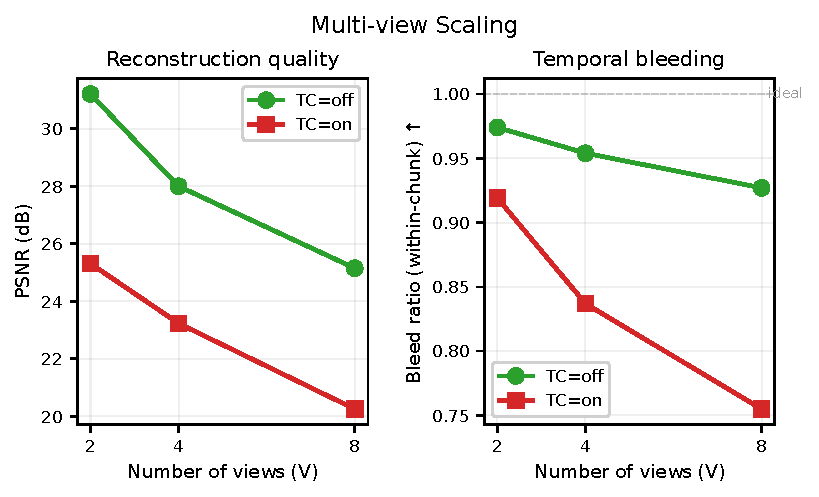
\includegraphics[width=0.95\linewidth]{figures/view_count.pdf}
\caption{Scaling the number of fused views at fixed latent width. Reconstruction quality and within-chunk bleed ratio both fall as $V$ grows, and the drop is steeper when temporal compression is also on --- more axes sharing the same 16 channels.}
\label{fig:view_count}
\end{figure}



\subsubsection{Resolution scaling}

The main matrix is at $128^2$ for throughput; $256^2$ and $512^2$ check that the joint-compression failure is not an artifact of the toy resolution. It is not: at $512^2$, E9b lands at 26.64~dB (Tab.~\ref{tab:res}), 1.14~dB below $256^2$ and only 1.33~dB above the 128px baseline. The $128{\to}256$ lift of ${+}2.47$~dB does not continue. LPIPS also worsens with resolution (0.082 $\to$ 0.102 $\to$ 0.170), consistent with more high-frequency identity detail sharing the same 16-channel latent. Bleed-W stays in the same band as 128px (0.904 vs.\ 0.919). Joint compression remains the binding constraint at every resolution we tested.

\begin{table}[t]
\centering
\caption{Resolution scaling under joint compression (fused, TC on, 16-ch).}
\label{tab:res}
\begin{tabular}{lrrrr}
\toprule
Resolution & PSNR $\uparrow$ & LPIPS $\downarrow$ & Bleed-W $\uparrow$ & XView sim \\
\midrule
128$^2$ (E1d)  & 25.31 & 0.082 & 0.919 & 0.920 \\
256$^2$ (E9a)  & 27.78 & 0.102 & 0.941 & 0.904 \\
512$^2$ (E9b)  & 26.64 & 0.170 & 0.904 & 0.904 \\
\bottomrule
\end{tabular}
\end{table}

\begin{figure}[t]
\centering
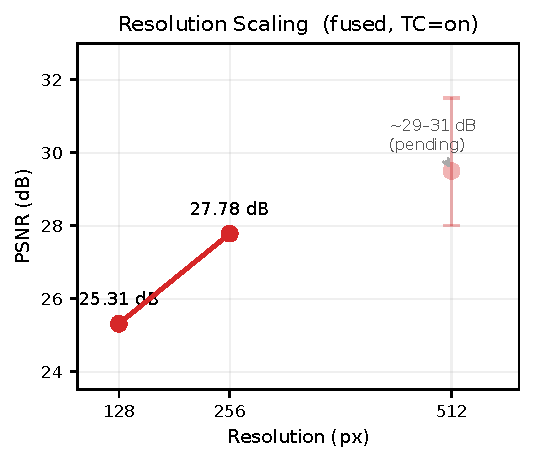
\includegraphics[width=0.62\linewidth]{figures/resolution_scaling.pdf}
\caption{PSNR vs resolution for fused TC=on. Quality rises from 128px to 256px, then falls back at 512px: the joint-compression failure is not a toy-resolution artifact.}
\label{fig:resolution}
\end{figure}



\subsubsection{Generalization pressure: training-set size}

We train the same fused+TC architecture on a single sequence, then one person, then all participants (one expression), and plot bleed ratio and ghosting against dataset size (Fig.~\ref{fig:datascale}). The prediction is that compression only breaks when it must generalize.

\begin{figure}[t]
\centering
\fbox{\parbox[c][4cm][c]{0.9\linewidth}{\centering
PLACEHOLDER Fig.~\ref{fig:datascale}: bleed ratio (within-chunk) and cross-view similarity\\
vs training-set size (single sequence / one person / all people), fused + TC config.\\
Expected: both diagnostics clean at single-sequence, degrading with dataset size.}}
\caption{Failure vs generalization pressure. The same architecture reconstructs a single sequence cleanly; artifacts appear as the training distribution grows.}
\label{fig:datascale}
\end{figure}



\subsection{Secondary ablations}
% [feedback] kept in the main text for now; referred to from the analysis above. Once all
% results exist these may move to the supplement.



\subsubsection{Loss configuration}

The default protocol uses no discriminator, perceptual weight $1.5$, and KL weight $10^{-6}$. We re-run the E1d setting (fused, TC on) with each discriminator layout and with lower/higher perceptual weight and a lower KL weight (Tab.~\ref{tab:loss}). \textbf{[RUNNING]} Protocol-matched jobs 37--42 are queued (5528048--5528053). Historical April/wandb numbers are not cited: they mixed batch sizes and used a LoRA checkpoint-load bug that left most of the backbone randomly initialized.

\begin{table}[t]
\centering
\caption{Loss configuration under joint compression (fused, TC on). Default row is E1d. Discriminator and weight arms are \textbf{[RUNNING]}.}
\label{tab:loss}
\begin{tabular}{lrrr}
\toprule
Loss config & PSNR $\uparrow$ & LPIPS $\downarrow$ & Bleed-W $\uparrow$ \\
\midrule
none, perc $1.5$, KL $10^{-6}$ (default) & 25.31 & 0.082 & 0.919 \\
\midrule
3D PatchGAN, views flattened            & \textbf{[RUNNING]} & --- & --- \\
joint 4D discriminator                  & \textbf{[RUNNING]} & --- & --- \\
3D PatchGAN, views stacked on channels  & \textbf{[RUNNING]} & --- & --- \\
\midrule
perceptual weight $0.5$                 & \textbf{[RUNNING]} & --- & --- \\
perceptual weight $3.0$                 & \textbf{[RUNNING]} & --- & --- \\
KL weight $10^{-7}$                     & \textbf{[RUNNING]} & --- & --- \\
\bottomrule
\end{tabular}
\end{table}


\subsubsection{LoRA rank}

We sweep rank $\{8,32,128\}$ at the E1c setting (fused, TC off), holding data and budget fixed. Rank 32 is the protocol default (31.21~dB). \textbf{[RUNNING]} Ranks 8 and 128 are jobs 43--44 (5528054--5528055).

\begin{table}[t]
\centering
\caption{LoRA rank at fused TC=off. Rank 32 is E1c; 8 and 128 are \textbf{[RUNNING]}.}
\label{tab:lora_rank}
\begin{tabular}{lrrr}
\toprule
LoRA rank & PSNR $\uparrow$ & LPIPS $\downarrow$ & XView sim \\
\midrule
8     & \textbf{[RUNNING]} & --- & --- \\
32 (default) & 31.21 & 0.044 & 0.907 \\
128   & \textbf{[RUNNING]} & --- & --- \\
\bottomrule
\end{tabular}
\end{table}


\subsubsection{Initialization strategy}
We compare a staged warm-start of the joint model from a temporal-compression checkpoint (with re-randomized view attention, the default) against joint training from Wan-pretrained weights only. Warm-start is marginally \emph{worse}: 25.86~dB without warm-start versus 25.31~dB with it, a ${-}0.55$~dB gap in favor of joint training from scratch ($\approx$3.5 SE above noise, borderline significant at one seed). The staged-curriculum hypothesis --- learn temporal first, then view --- is not supported. A plausible explanation is that the temporal checkpoint anchors the encoder to a local minimum that is suboptimal for joint learning, whereas training from scratch allows both axes to co-adapt. Given the small gap and a single seed, this result warrants caution; it does not affect any other conclusion.


\subsubsection{Pre-fusion encoder LoRA}

The default places LoRA only after fusion (bottleneck and decoder). Adding LoRA on the frozen per-view encoder stem ($E_{\mathrm{pre}}$) tests whether the joint-compression failure is an under-adapted encoder or a bottleneck after fusion (Tab.~\ref{tab:lora_before}). \textbf{[RUNNING]} Jobs 45 (E1d) and 46 (E1c) are 5528056--5528057. If pre-fusion LoRA does not close the joint-compression gap, the information is missing from the latent, not from the stem.

\begin{table}[t]
\centering
\caption{Pre-fusion encoder LoRA. Default is after-only. Both ``before+after'' arms are \textbf{[RUNNING]}.}
\label{tab:lora_before}
\begin{tabular}{llrrr}
\toprule
TC & LoRA placement & PSNR $\uparrow$ & LPIPS $\downarrow$ & Bleed-W $\uparrow$ \\
\midrule
off & after only (E1c)     & 31.21 & 0.044 & 0.974 \\
off & before + after       & \textbf{[RUNNING]} & --- & --- \\
\midrule
on  & after only (E1d)     & 25.31 & 0.082 & 0.919 \\
on  & before + after       & \textbf{[RUNNING]} & --- & --- \\
\bottomrule
\end{tabular}
\end{table}











\section{Discussion}

This section discusses the main findings and considers implications and potential applications of this work.

\subsection{Capacity}

In our setup the Wan latent has 16 channels per $8{\times}8{\times}4$ pixel block, i.e.\ $3{\cdot}8{\cdot}8{\cdot}4/16 = 48\times$ compression. Fusing $V{=}2$ views into one latent doubles this to $96\times$; $V{=}4$ yields $192\times$. For comparison, Emu \cite{dai2023emu} needed a widening from 4 to 16 channels just to hold fine detail at $48\times$-equivalent rates, and LTX-Video \cite{hacohen2024ltx} uses 128 channels at $192\times$. Our setting demands roughly 2--4$\times$ the information density of the pretrained latent at fixed width. The observed failure is exactly what rate exhaustion predicts: the decoder regresses to the conditional mean along whichever axis was compressed, showing up as ghosting (the view mean) and bleeding (the temporal mean).

The latent-width ablation (Tab.~\ref{tab:width}) provides the positive test: widening from 16 to 32 channels (${+}2.40$~dB) is the single largest isolated gain in the study, larger than any 16-channel temporal intervention. Widening to 64 channels adds only 0.01~dB over 32, suggesting that the $32{\to}64$ doubling hits a secondary bottleneck, likely the still-frozen strided temporal convolutions. At 32 channels the widened model matches the \emph{rate} of the per-view TC reference (both $36\times$) but remains 3.79~dB below it. Combining the 32-channel latent with the temporal-difference loss is additive (29.56~dB, ${+}4.25$ vs.\ ${+}4.23$ expected) and cuts that leftover gap to 1.94~dB, so width and temporal supervision address independent constraints. Capacity is therefore \emph{necessary} but not solely sufficient: the frozen temporal convolutions are a secondary constraint. A purpose-built 4D tokenizer with trained temporal convolutions and 32--64 channels would likely close the remaining gap.

Two further observations support the capacity reading. First, self-attention and Conv3d fusion, and all five view-conditioning variants, perform equivalently (max spread 0.43~dB and 0.32~dB respectively): if information does not fit the latent, no operator recovers it. Second, what fails first under joint compression is high-frequency identity detail --- nuanced facial appearance, fine texture --- precisely the detail class that widening image latents from 4 to 16 channels was needed to preserve \cite{dai2023emu}.

\subsection{Bottleneck: Encoder-side latent}

The decoder side works: per-view LoRA and embeddings reliably disambiguate views from a shared latent, and the conditioning mechanism is insensitive. The information is missing, not mis-decoded. The encoder-side latent would need to hold more than it can. The decoder can emit distinct views, but the fixed-width latent cannot carry them under joint compression. Post-hoc fixes --- embeddings, residual decoders, auxiliary losses --- cannot recover information: everything that operates after the bottleneck failed.

\subsection{Implications and Applications}

Designing a 4D tokenizer may require scaling latent width with the number of compressed axes --- \cite{chen2024deep, hacohen2024ltx} suggest roughly proportional scaling --- so a 4D VAE wants 32--64 channels, which requires pretraining or heavy finetuning, not adapters. Our width ablation is the adapter-scale version of exactly this recipe. A second design is to keep view identity out of the latent: compress only shared content and carry view as decoder conditioning. Our per-view LoRA is the adapter-scale version; a real system would train it. A third design is asymmetric: compress time natively, keep views uncompressed but consistent via cross-view attention, matching what 4D diffusion systems converged to \cite{xie2024sv4d, shao2024human4dit}.


\section{Conclusion}

We extended a pretrained 3D video VAE to multi-view video with zero-initialized multi-view self-attention fusion and per-view low-rank decoding, preserving the pretrained latent distribution and remaining compatible with unconditional sampling. On multi-view facial video, the fixed 16-channel latent absorbs either $4\times$ temporal compression or the fused view axis, but not both. Joint compression exhausts the latent's capacity and the decoder regresses to means, producing cross-view ghosting and intra-chunk temporal bleeding. The latent-width ablation turns the capacity claim into a tested one: widening from 16 to 32 channels recovers 2.40~dB under joint compression, the single largest isolated improvement in the study. Combining that widening with a temporal-difference loss is additive (29.56~dB, ${+}4.25$ vs.\ ${+}4.23$ expected), leaving a 1.94~dB gap to the per-view temporal-compression reference. This directly confirms the rate interpretation and matches the width-compression scaling observed in DC-AE \cite{chen2024deep} and LTX-Video \cite{hacohen2024ltx}, extended to the view axis. Future 4D tokenizers should either scale latent capacity with the number of compressed axes (32--64 channels for joint view and temporal compression) or keep view identity out of the latent and carry it as decoder conditioning; the per-view LoRA path studied here is the adapter-scale version of the latter.

\section{Limitations}

We compressed 9-frame clips --- rate pressure grows with $T$, so longer clips could shift conclusions --- and 2--8 frontal views, not the full rig. We tried one backbone family (Wan 2.1); the chunked-cache specifics of the temporal path are Wan's, and other causal video VAEs may fail differently. The training budget is adapter-scale: conclusions hold for LoRA-based adaptation of a frozen backbone; full pretraining at 4D scale could move the capacity wall, and that experiment is exactly what this study argues one should budget for. Downstream generation is untested: we evaluate the latent by reconstruction, and whether a diffusion model samples well from the fused latent is future work. In particular the widened latents are validated for reconstruction only, and wider latents are known to be harder to sample from \cite{yao2025vavae}. Object-centric capture is a requirement, not a convenience: our motivation and results presuppose largely overlapping fields of view (studio head capture, white background). For non-object-centric multi-view data the view axis carries new content by construction, there is little redundancy to compress, and the approach does not apply.


% ============================================================
% Supplementary material
% ============================================================
\clearpage
\appendix
\section*{Supplementary Material}

\subsection*{A. Validation split}

% [feedback] val subject selection moved here from the main text
Ten participants are held out entirely and never seen in training; all reported metrics are computed on them: p018, p030, p038, p085, p097, p124, p175, p226, p227, p240. The split is fixed once and used identically by every run. Qualitative validation panels always show the first three val clips in sorted dataset order in every run and every arm.

\subsection*{B. Preprocessing details}

Cameras are the 8 frontal and upper-row serials of the 16-camera rig. The temporal pipeline goes from 73~fps to a 24~fps subsample, then uniformly selects $T{=}9$ frames per sequence window. Per-camera color correction uses the matrices shipped with the dataset. We center-square-crop to $\min(H,W)$ and bilinearly resize to the target resolution. Background removal uses RobustVideoMatting \cite{lin2022robust}, composited on white. Tensors are stored as $[V, T, C, H, W]$ uint8 in $[0,1]$, batched as $[B, V, C, T, H, W]$, and rescaled to $[-1,1]$ at load time.

\subsection*{C. Training infrastructure}

Each run uses one L40S GPU, bf16, and gradient checkpointing on the per-view encoder and decoder body. Effective batch 64 is realized via micro-batch times accumulation; an OOM ladder re-balances the product, never the total. Jobs are chained in 18h slices with automatic checkpoint resume, so every arm has an identical optimizer-update budget.

\subsection*{D. Additional tables and figures}

The supplement will include per-view (instead of view-averaged) metric tables for every experiment, full per-frame PSNR profiles and anchor-drift ($|f_k-f_0|$) curves for all arms, and a side-by-side GT versus reconstruction video for all arms on the same fixed participants.
